\documentclass[10pt,a4paper]{article}

% --- Layout ---
\usepackage[margin=2cm, top=2.5cm]{geometry}
\usepackage{parskip}
\usepackage{microtype}

% --- Math ---
\usepackage{amsmath, amssymb}

% --- Tables ---
\usepackage{booktabs}
\usepackage{array}
\usepackage{tabularx}

% --- Graphics ---
\usepackage{graphicx}
\usepackage{float}

% --- Sections ---
\usepackage{titlesec}
\titleformat{\section}{\large\bfseries}{}{0em}{}[\titlerule]
\titleformat{\subsection}{\normalsize\bfseries}{}{0em}{}
\titlespacing{\section}{0pt}{1.4ex plus .2ex}{0.5ex}
\titlespacing{\subsection}{0pt}{0.9ex}{0.3ex}

% --- Lists ---
\usepackage{enumitem}
\setlist{noitemsep, topsep=2pt, parsep=0pt}

% --- Colours and links ---
\usepackage{xcolor}
\definecolor{linkblue}{rgb}{0.08,0.18,0.55}
\definecolor{midgray}{gray}{0.40}
\definecolor{flagred}{rgb}{0.72,0.11,0.11}
\usepackage{hyperref}
\hypersetup{colorlinks=true, urlcolor=linkblue, linkcolor=black, citecolor=midgray}

% --- tcolorbox for callout ---
\usepackage{tcolorbox}

% --- Header / Footer ---
\usepackage{fancyhdr}
\pagestyle{fancy}
\fancyhf{}
\lhead{\small\textbf{Dry Lab Deliverable: Task 6} \textbullet{} Eton iGEM 2026}
\rhead{\small Aaran Nihalani}
\cfoot{\small\thepage}
\renewcommand{\headrulewidth}{0.3pt}
\renewcommand{\footrulewidth}{0pt}

\begin{document}

% --- Title block ---
\begin{center}
  {\LARGE\bfseries Cross-Reactivity Specificity Matrix}\\[0.15em]
  {\normalsize Task 6 \textbullet{} Dry Lab Deliverable}\\[0.08em]
  {\small Aaran Nihalani \textbullet{} Eton iGEM 2026 \textbullet{} \today}
\end{center}
\vspace{0.3em}\hrule\vspace{0.5em}

A multiplexed electrochemical biosensor requires that each substrate motif is cleaved
selectively by its target protease and not by any other panel member. This report
presents a quantitative cross-reactivity specificity matrix for the six-protease diagnostic
panel, computed from position-specific scoring matrices (PSSMs) built from all confirmed
cleavage events in the MEROPS substrate database. Panel motifs for MMP-8, MMP-9, NE,
and Fecal are the top-ranked candidates from the Task~7 ML substrate predictor; MMP14
uses the validated electrochemical sensor motif; FAP uses the Edosada literature reference.
Of 30 off-diagonal pairs, 23 are orthogonal (score $< 0.05$) and 7 are flagged
($\geq 0.20$).

% ============================================================
\section{Task 6: Cross-Reactivity Specificity Matrix}
% ============================================================

\subsection{Data Source and PSSM Construction}

Confirmed cleavage-site sequences were downloaded from the MEROPS bulk release
(\texttt{Substrate\_search.txt}, accessed July 2026; 108,183 entries total). Records were
filtered to the six MEROPS identifiers in Table~\ref{tab:training}. For each of the eight
P4--P4' positions, amino acid frequencies were computed with a Laplace pseudocount of 0.5
and converted to log$_2$ odds against Swiss-Prot background frequencies (Robinson \&
Robinson 1991), yielding one $8 \times 20$ PSSM per protease. The fecal serine protease
PSSM pools three sub-entries (trypsin-1, chymotrypsin~B, elastase-1); it is dominated by
trypsin-1 (18,131 of 18,251 entries), which confers strong Arg/Lys specificity at P1.
FAP has only 2 unique cleavage windows in MEROPS: its PSSM is statistically non-informative
and all FAP-related values are flagged throughout.

\vspace{0.4em}
\begin{table}[H]
\centering
\begin{tabularx}{\textwidth}{@{}p{2.2cm} p{2.2cm}
  >{\raggedleft\arraybackslash}p{2.4cm}
  p{2.0cm} X@{}}
\toprule
\textbf{Protease} & \textbf{MEROPS ID} & \textbf{Unique windows} & \textbf{Confidence} & \textbf{Notes} \\
\midrule
MMP14  & M10.014     &    129 & medium & MT1-MMP \\
MMP-8  & M10.002     &     96 & medium & Neutrophil collagenase \\
MMP-9  & M10.004     &    341 & high   & Gelatinase B \\
NE     & S01.131     &    327 & high   & Neutrophil elastase \\
Fecal  & S01.151/2/3 & 18,251 & high   & Trypsin-1 dominated \\
FAP    & S09.007     &      2 & \textcolor{flagred}{\textbf{unusable}} & See \S\ref{sec:negself} \\
\bottomrule
\end{tabularx}
\caption{MEROPS training data per protease. Unique windows after 3-letter-to-1-letter
conversion, standard-amino-acid filtering, and deduplication.}
\label{tab:training}
\end{table}

\subsection{Panel Motifs}

Table~\ref{tab:motifs} lists the six motifs evaluated as column vectors. MMP-8, MMP-9,
NE, and Fecal use the top-ranked candidates from the Task~7 ML substrate predictor (this
work). MMP14 retains the experimentally validated sensor motif SGRSENIR. FAP uses the
Edosada literature reference because the Task~7 FAP model is degenerate ($n=2$ positives).

\vspace{0.4em}
\begin{table}[H]
\centering
\begin{tabularx}{\textwidth}{@{}p{2.5cm} p{2.2cm} X p{3.2cm}@{}}
\toprule
\textbf{Protease} & \textbf{Motif} & \textbf{Source} & \textbf{Status} \\
\midrule
MMP14 & \texttt{SGRSENIR} & Ohuchi et al.\ 1997 & Fixed, validated \\
MMP-8 & \texttt{KSQFLQGT} & Task 7 ML prediction & LR AUROC 0.773, $S = 2.02$ \\
MMP-9 & \texttt{GAPPVQAP} & Task 7 ML prediction & LR AUROC 0.774, $S = 2.39$ \\
NE    & \texttt{PETISLPP} & Task 7 ML prediction & LR AUROC 0.825, $S = 17.9$ \\
Fecal & \texttt{DLPRALDQ} & Task 7 ML prediction & LR AUROC 0.938, $S = 1.98$ \\
FAP   & \texttt{GPRFPIGS} & Edosada et al.\ 2006 & Literature; ML unreliable \\
\bottomrule
\end{tabularx}
\caption{Panel motifs used as column vectors in the specificity matrix. $S$ = ML
selectivity index (target probability / maximum competitor probability) from Task~7.}
\label{tab:motifs}
\end{table}

\subsection{Specificity Matrix}

Each cell in Table~\ref{tab:specificity} is the PSSM log$_2$-odds score of the column
motif under the row protease's matrix, divided by the absolute self-score (so the
diagonal reference is $\pm 1.00$). Values $\geq 0.20$ are {\color{flagred}\textbf{flagged}};
values $< 0.05$ in absolute magnitude are considered orthogonal.

\vspace{0.4em}
\begin{table}[H]
\centering
\setlength{\tabcolsep}{10pt}
\begin{tabular}{@{}l c c c c c c@{}}
\toprule
\textbf{Protease} & \textbf{MMP14} & \textbf{MMP-8} & \textbf{MMP-9} & \textbf{NE} & \textbf{Fecal} & \textbf{FAP} \\
\midrule
MMP14 & $-1.00^{\dagger}$ & \textcolor{flagred}{\textbf{0.86}} & \textcolor{flagred}{\textbf{0.54}} & $-1.72$ & $-0.12$ & $-0.76$ \\
MMP-8 & $-0.41$ & $1.00$ & \textcolor{flagred}{\textbf{0.70}} & $-0.89$ & $-0.38$ & \textcolor{flagred}{\textbf{0.52}} \\
MMP-9 & $-0.59$ & \textcolor{flagred}{\textbf{0.48}} & $1.00$ & $-0.62$ & $-0.49$ & \textcolor{flagred}{\textbf{0.64}} \\
NE    & $-0.82$ & $-0.39$ & $-0.11$ & $1.00$ & $-0.10$ & $-0.74$ \\
Fecal & $-1.64$ & $-0.90$ & $-1.08$ & $-0.98$ & $1.00$ & $-1.91$ \\
FAP   & $-1.15$ & \textcolor{flagred}{\textbf{0.42}} & $0.02$ & $-1.20$ & $-0.62$ & $-1.00^{\dagger}$ \\
\bottomrule
\end{tabular}
\\[0.4em]
{\small $^{\dagger}$Negative self-score: motif scores below Swiss-Prot background
under its own PSSM (see \S\ref{sec:negself}).}
\caption{Normalised cross-reactivity specificity matrix. Rows: proteases (PSSM used for
scoring). Columns: motifs being scored. Diagonal = self-score reference ($\pm 1.00$).
\textcolor{flagred}{\textbf{Bold red}}: $\geq 0.20$ (flagged). 23 of 30 off-diagonal
pairs are orthogonal ($< 0.05$).}
\label{tab:specificity}
\end{table}

\begin{figure}[H]
  \centering
  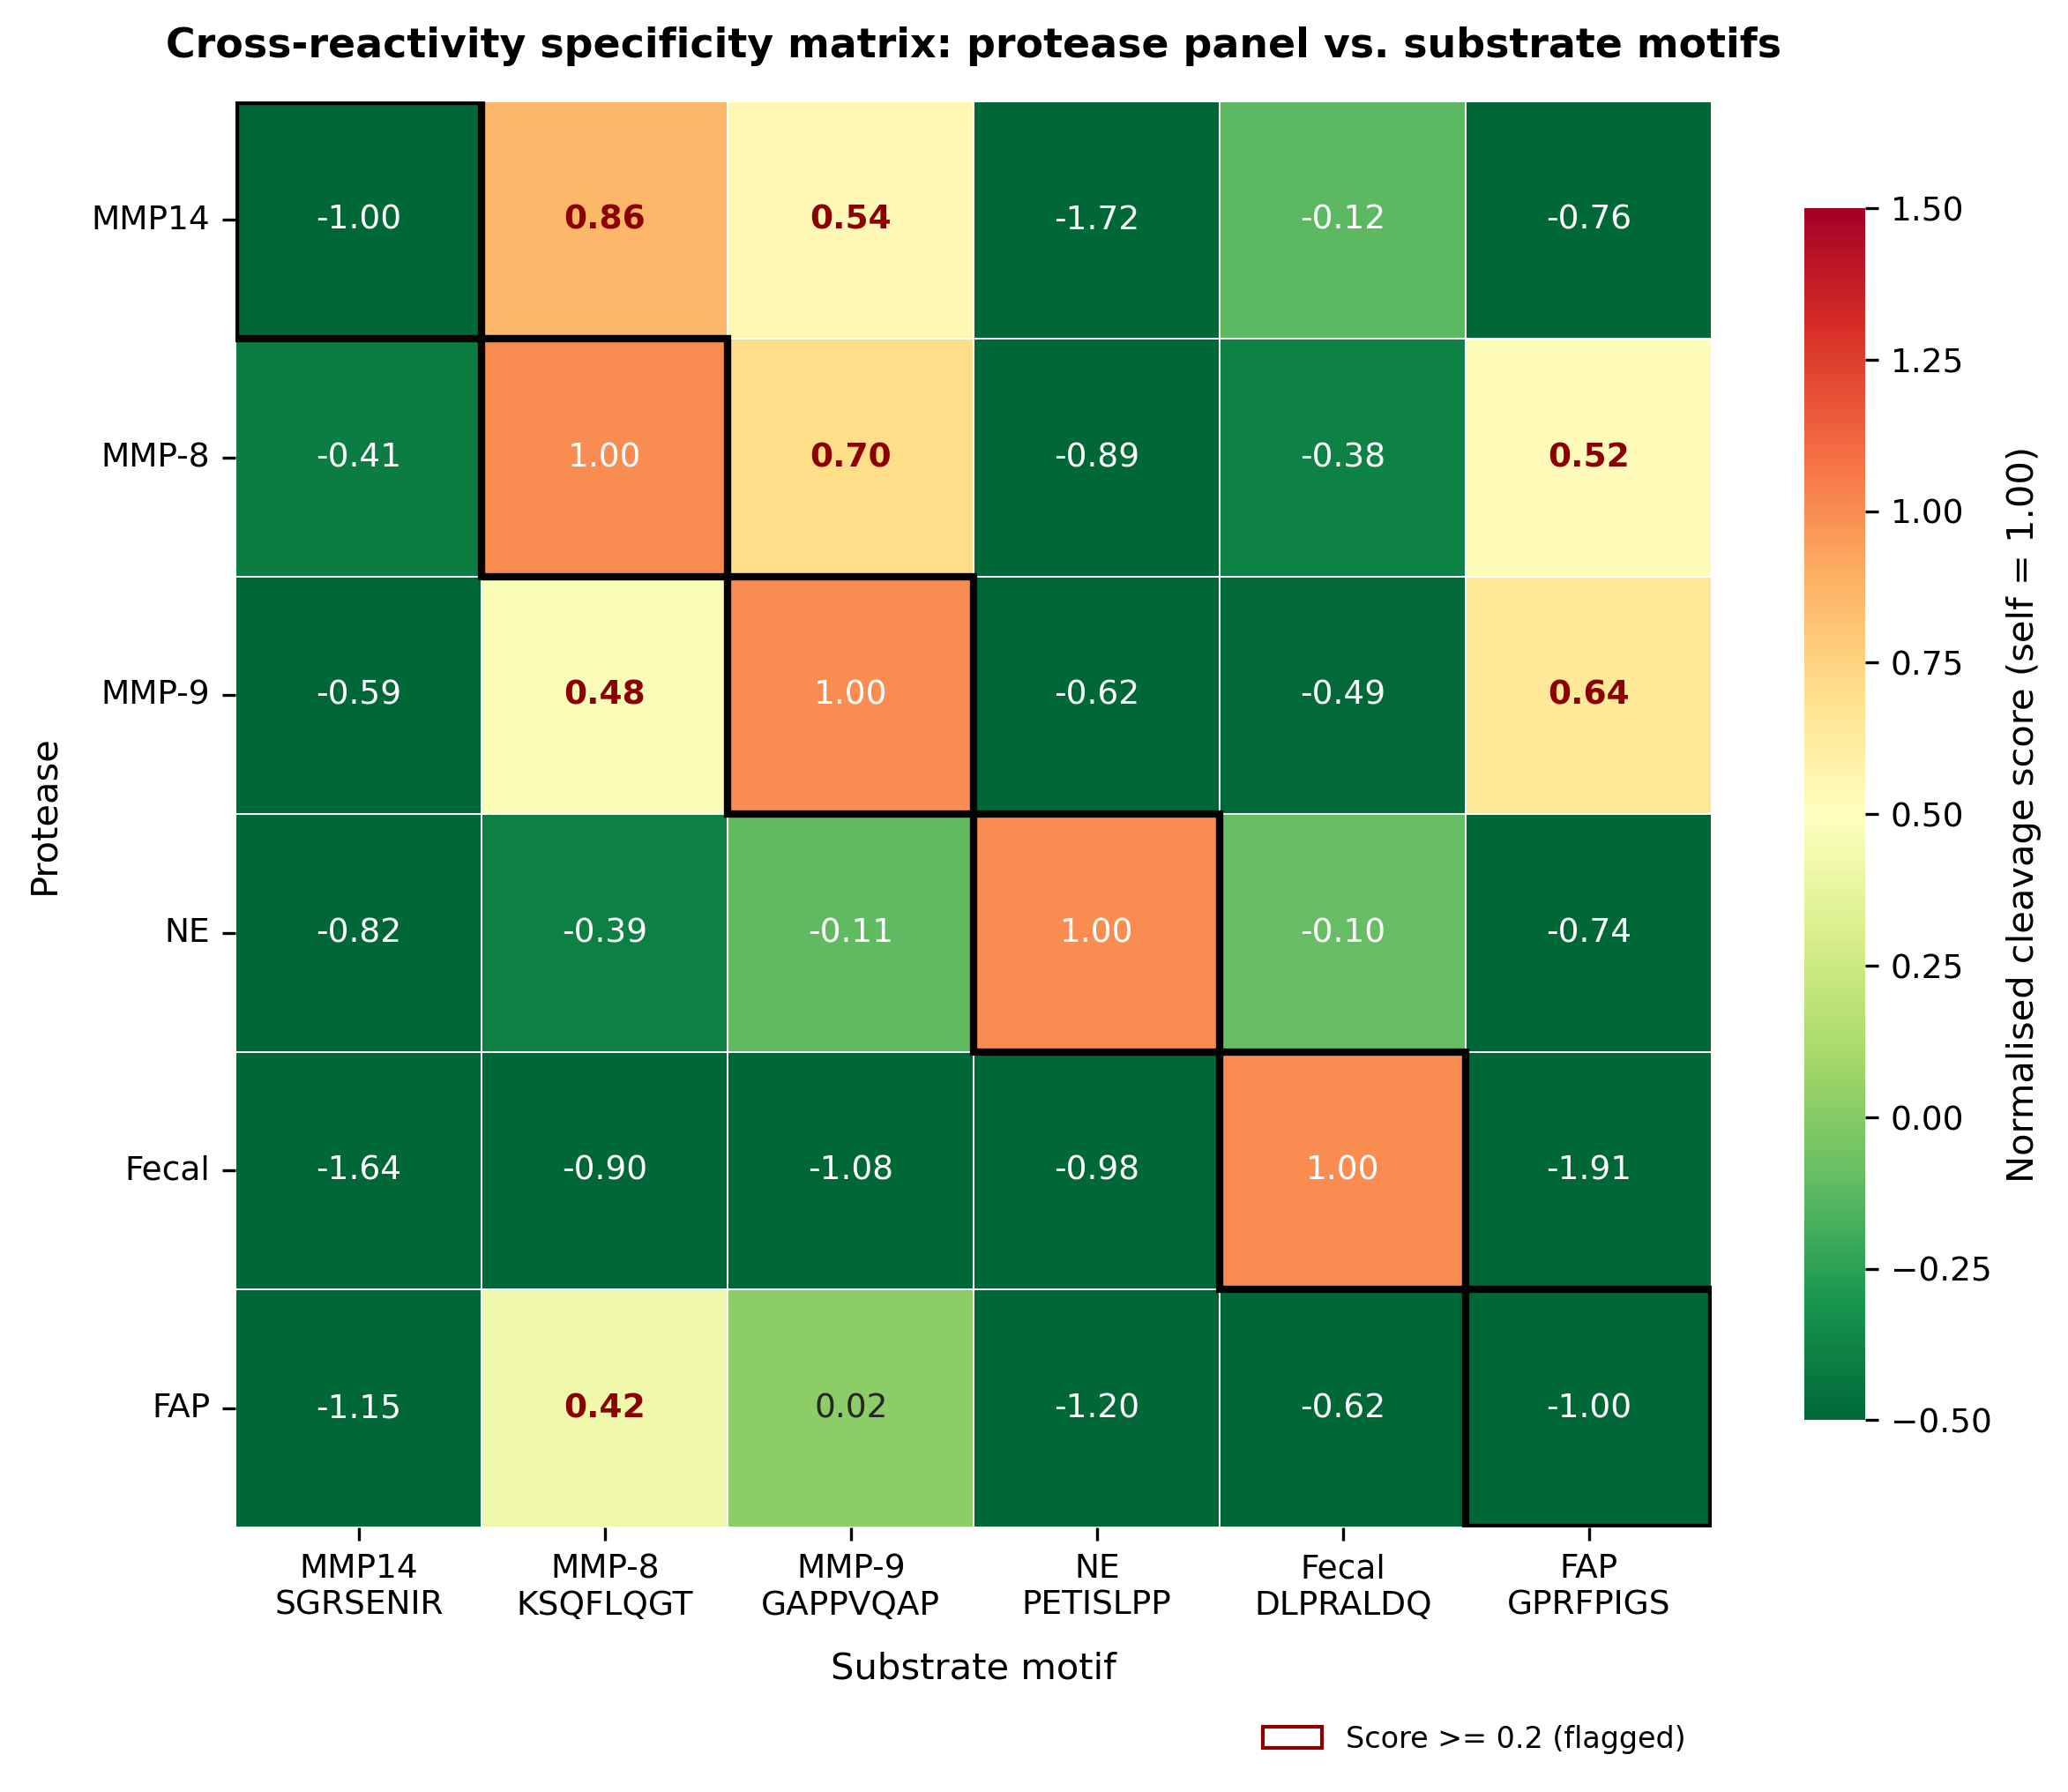
\includegraphics[width=0.96\textwidth]{figures/fig_specificity_heatmap.png}
  \caption{Specificity matrix heatmap. Rows: proteases; columns: substrate motifs.
  Colour scale: \texttt{RdYlGn\_r} (red: cross-reactive, green: orthogonal). Diagonal
  cells are outlined in black. Off-diagonal values $\geq 0.20$ are annotated in bold
  red. Panel motifs are indicated in column headers.}
  \label{fig:heatmap}
\end{figure}

\subsection{Flagged Pairs}
\label{sec:flagged}

Seven of 30 off-diagonal pairs exceed the 0.20 threshold. They fall into two distinct
groups.

\textbf{Intra-MMP cross-reactivity (four pairs).}
The pairs MMP14$\times$KSQFLQGT (0.86), MMP14$\times$GAPPVQAP (0.54),
MMP-8$\times$GAPPVQAP (0.70), and MMP-9$\times$KSQFLQGT (0.48) all reflect the
shared M10A active-site architecture. All three gelatinolytic/collagenolytic MMPs use
a Zn$^{2+}$ catalytic mechanism with a deep hydrophobic S1' pocket accepting Phe, Leu,
and Ile, and a broad S2 subsite. The ML-predicted motifs KSQFLQGT and GAPPVQAP were
optimised for cleavage probability by MMP-8 and MMP-9 respectively; because the M10A
pocket geometry is shared, both motifs are also well-tolerated by the other panel MMPs.
This is an intrinsic constraint of the MMP subfamily: motifs that maximise individual
cleavage efficiency will inevitably retain some cross-reactivity with family members.
Note that the MMP-8 and MMP-9 ML selectivity indices ($S = 2.02$ and $2.39$) already
reflect this; they are real but moderate.

\textbf{FAP-related artefacts (three pairs).}
MMP-9$\times$GPRFPIGS~(0.64), MMP-8$\times$GPRFPIGS~(0.52), and
FAP$\times$KSQFLQGT~(0.42) all involve the FAP literature motif (GPRFPIGS) or the FAP
PSSM, both of which are built from 2 MEROPS entries and have no statistical power.
These values are not interpretable as genuine cross-reactivity and are excluded from any
sensor design recommendation.

\subsection{Negative Self-Scores and MMP14 SGRSENIR}
\label{sec:negself}

MMP14 (SGRSENIR, raw self-score $= -3.81$) and FAP (GPRFPIGS, raw self-score $= -3.47$)
have negative diagonal values, meaning the motif scores below the Swiss-Prot background
under its own protease's PSSM. For MMP14, this reflects a documented divergence between
natural ECM substrates in MEROPS (collagen, fibronectin: enriched for Pro, Gly, and Leu
at P1') and the SGRSENIR biosensor motif (derived from the proMMP-2 autolytic site,
enriched for Ser and Arg). SGRSENIR is experimentally validated as an MMP14 substrate
($k_{\text{cat}}/K_M = 5.5 \times 10^4\ \text{M}^{-1}\text{s}^{-1}$; Ohuchi et al.\
1997) and has been deployed in working electrochemical sensors. The PSSM mismatch
reflects a MEROPS ascertainment bias towards natural ECM substrates and is not a
functional deficiency of the sensor. For FAP, the negative self-score is simply noise
from 2 database entries. In both cases the diagonal is normalised to $-1.00$ and
interpreted accordingly.

\begin{tcolorbox}[colback=gray!7, colframe=gray!40, boxrule=0.4pt,
  arc=2pt, left=6pt, right=6pt, top=4pt, bottom=4pt]
  \textbf{Summary.} The serine protease block (NE, Fecal) is cleanly orthogonal to all
  three panel MMPs: every cross-reactivity score in the NE and Fecal rows is negative
  (below Swiss-Prot background), and the MMP rows score NE and Fecal motifs at
  $\leq -0.10$. This is the strongest structural result: the protease class boundary
  between serine and metalloprotease families is sufficient to ensure selectivity without
  motif optimisation. Within the M10 metalloproteinase subfamily, all three MMPs show
  mutual cross-reactivity ($0.48$--$0.86$) with the ML-predicted motifs. The NE
  candidate (\texttt{PETISLPP}) achieves an ML selectivity of 17.9, making it the
  highest-confidence motif in the panel. FAP requires either additional substrate data
  or a structure-based approach before a reliable specificity assessment is possible.
\end{tcolorbox}

\end{document}
